\subsection{Pruebas y resultados}
	\subsubsection{Hormiga de Langton Original}
		\begin{figure}[H]
			\begin{center}
				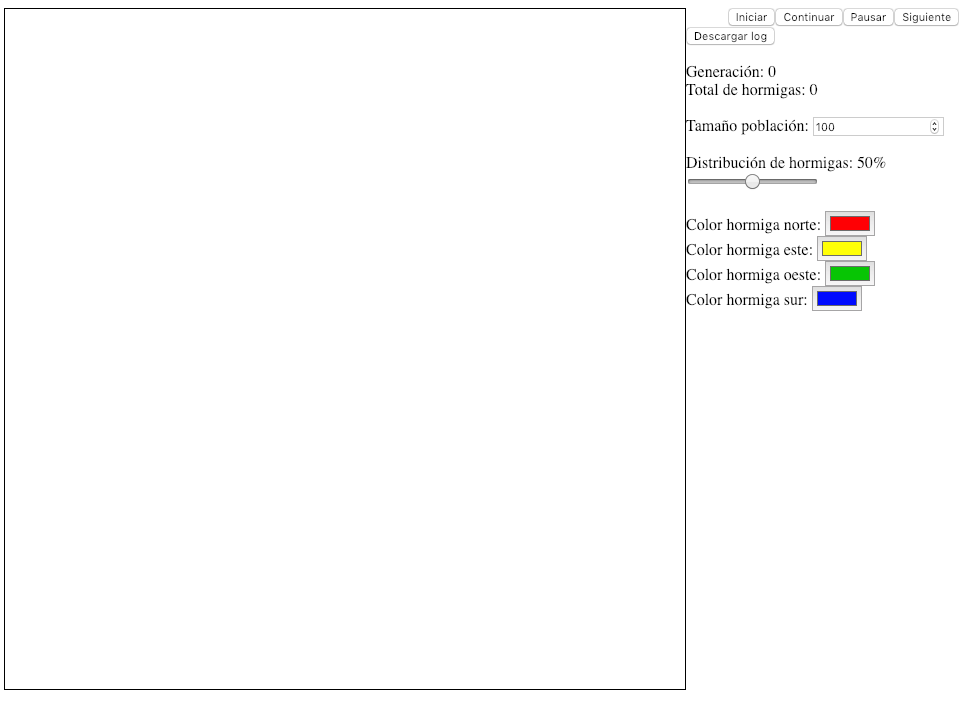
\includegraphics[scale=.3]{HL/img/interfaz.png}
				\caption{Interfaz gráfica del programa}
				\label{fig:hl1}
			\end{center}
		\end{figure}

		\begin{figure}[H]
			\begin{center}
				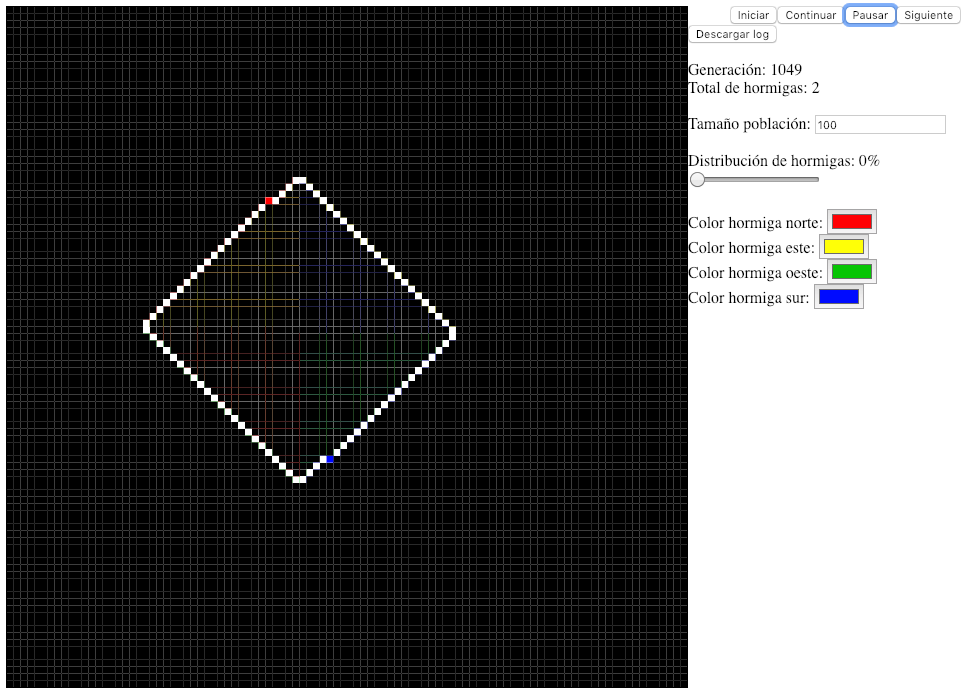
\includegraphics[scale=.3]{HL/img/dos.png}
				\caption{Dos hormigas agregadas por el usuario después de 1000 generaciones}
				\label{fig:hl1}
			\end{center}
		\end{figure}

		\begin{figure}[H]
			\begin{center}
				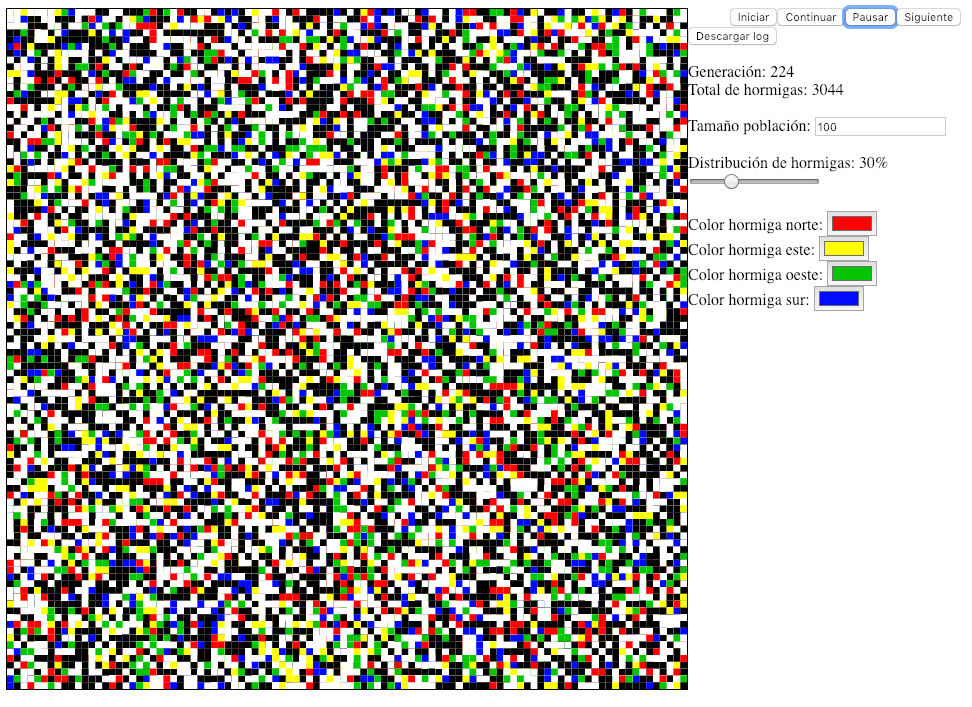
\includegraphics[scale=.3]{HL/img/varias.png}
				\caption{Varias hormigas generadas mediante la distribución}
				\label{fig:hl1}
			\end{center}
		\end{figure}

		\begin{figure}[H]
			\begin{center}
				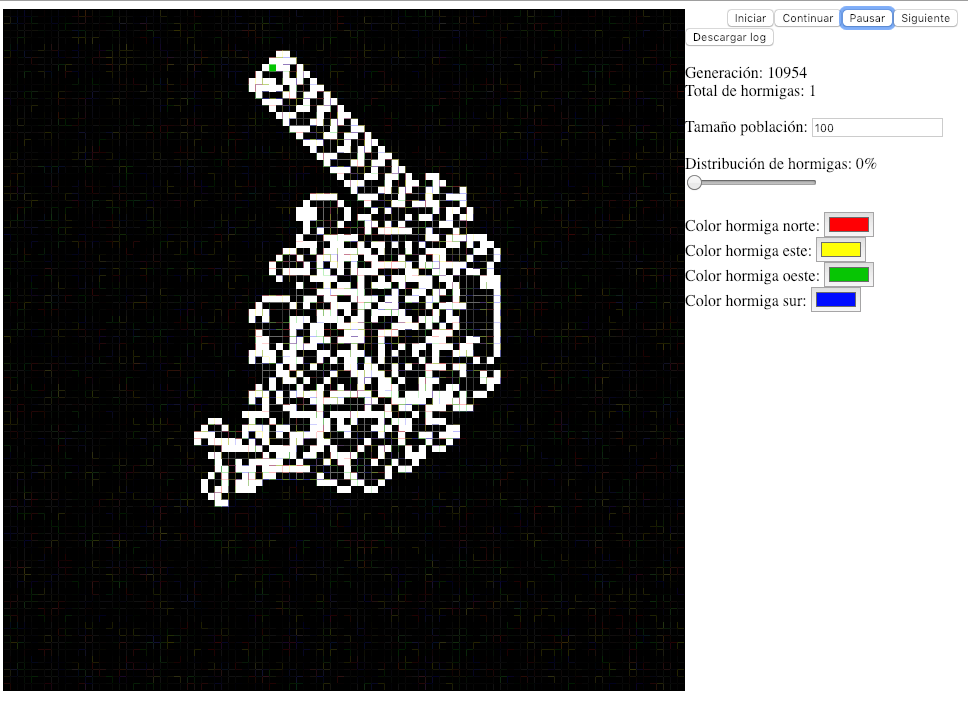
\includegraphics[scale=.3]{HL/img/hormiga.png}
				\caption{Hormiga repitiendo un patrón después de 10,000 generaciones}
				\label{fig:hl1}
			\end{center}
		\end{figure}

	\subsection{Hormiga de Langton Modificada}
		\begin{figure}[H]
			\begin{center}
				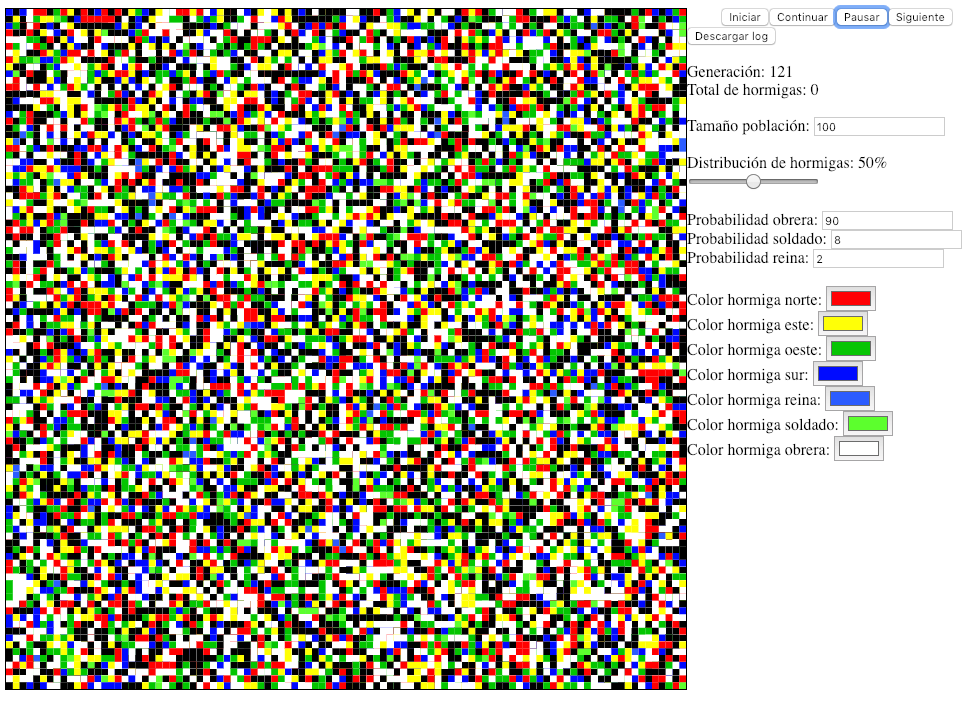
\includegraphics[scale=.3]{HL/img/mod1-1.png}
				\caption{Colonia con probabilidades por defecto}
				\label{fig:hl1}
			\end{center}
		\end{figure}

		\begin{figure}[H]
			\begin{center}
				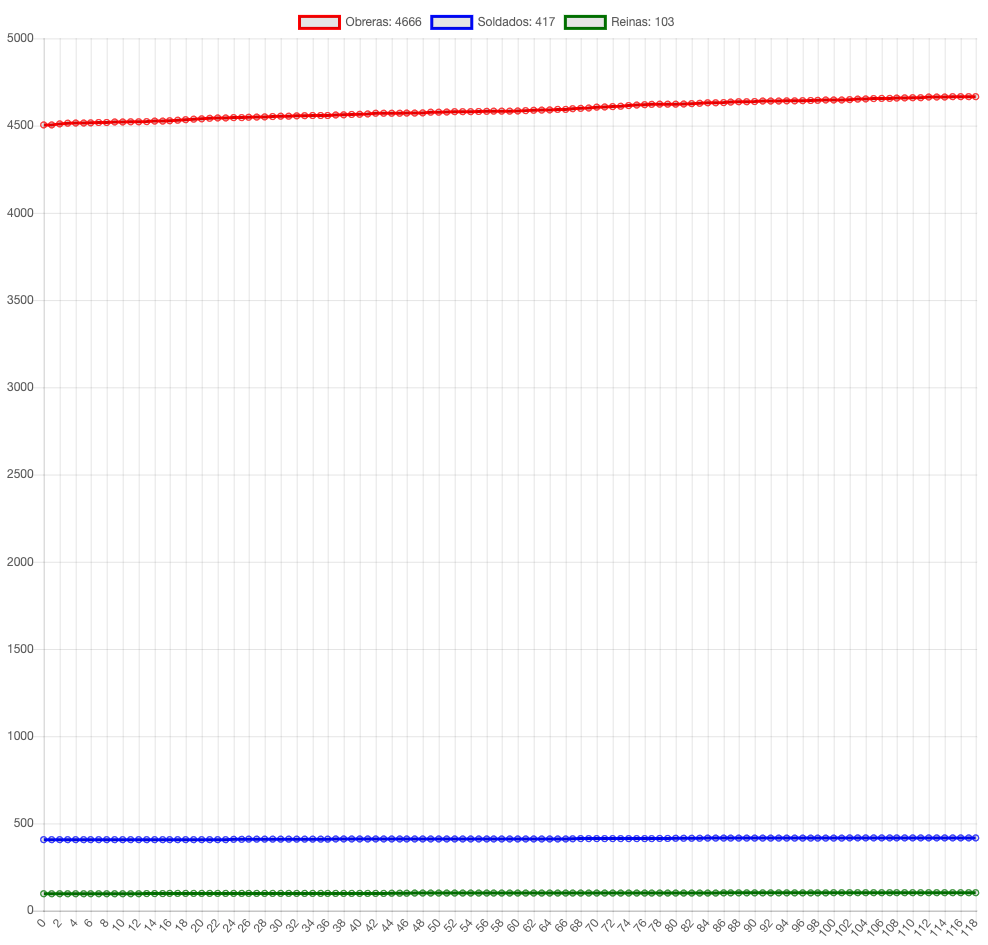
\includegraphics[scale=.24]{HL/img/mod1-2.png}
				\caption{Gráfica de la colonia anterior}
				\label{fig:hl1}
			\end{center}
		\end{figure}

		\begin{figure}[H]
			\begin{center}
				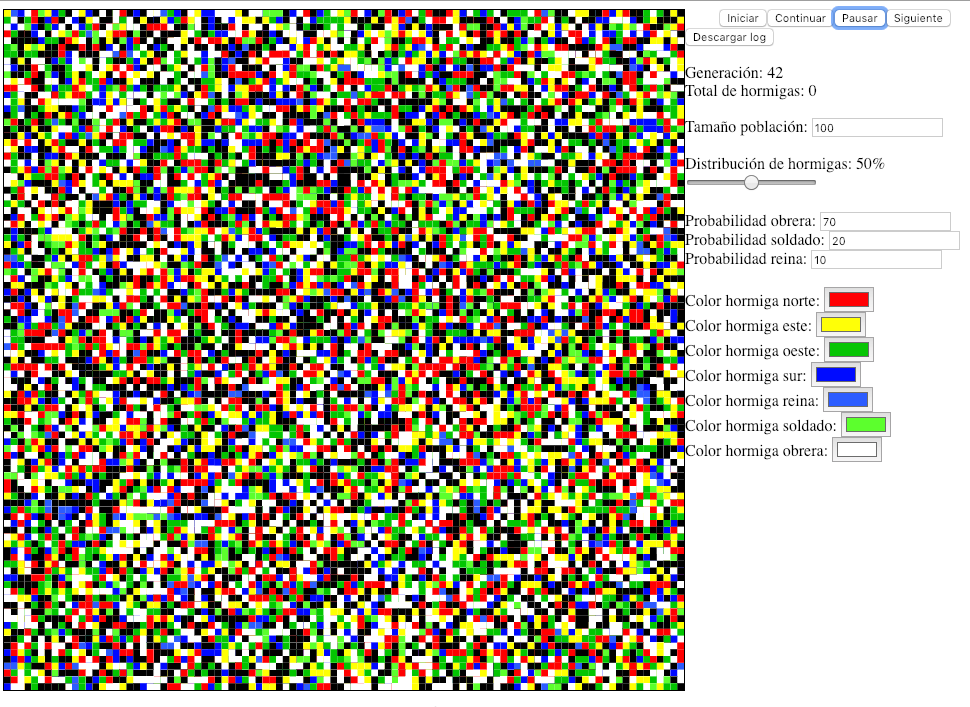
\includegraphics[scale=.3]{HL/img/mod2-1.png}
				\caption{Probabilidades de 70,20 y 10}
				\label{fig:hl1}
			\end{center}
		\end{figure}

		\begin{figure}[H]
			\begin{center}
				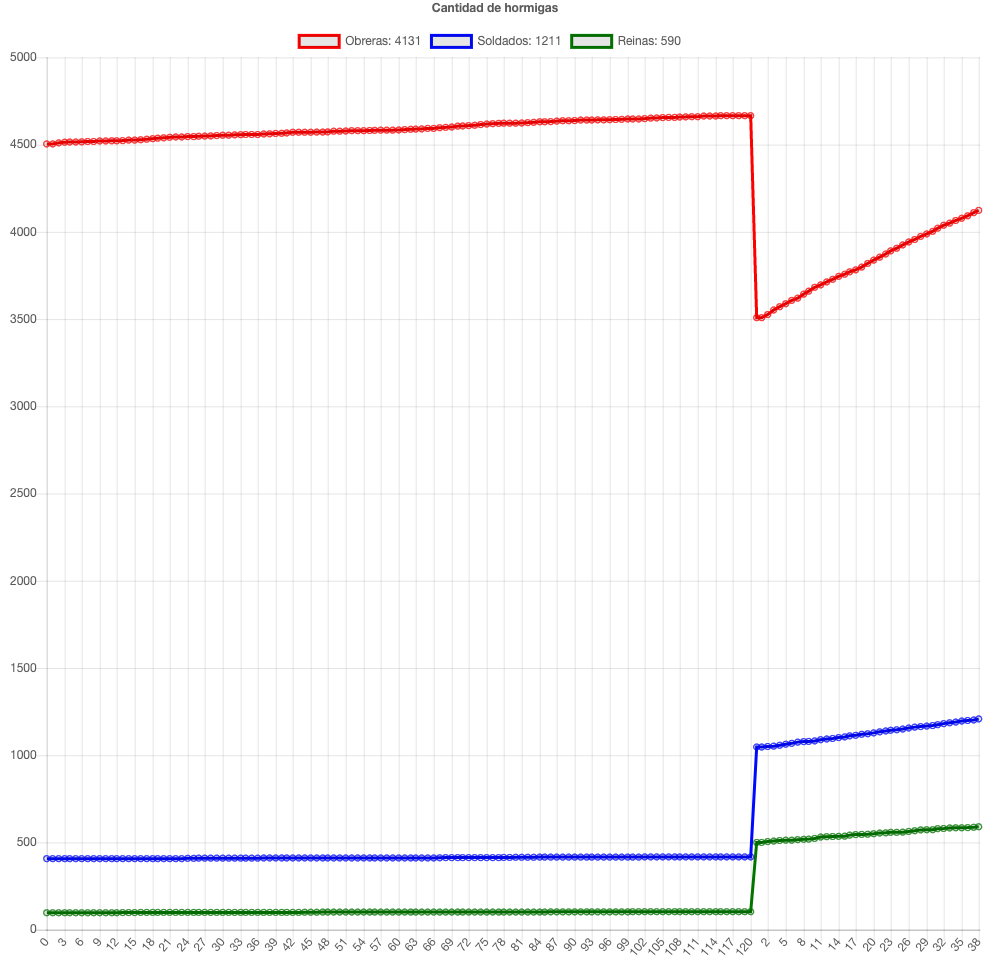
\includegraphics[scale=.24]{HL/img/mod2-2.png}
				\caption{Gráfica de la colonia anterior}
				\label{fig:hl1}
			\end{center}
		\end{figure}

		\begin{figure}[H]
			\begin{center}
				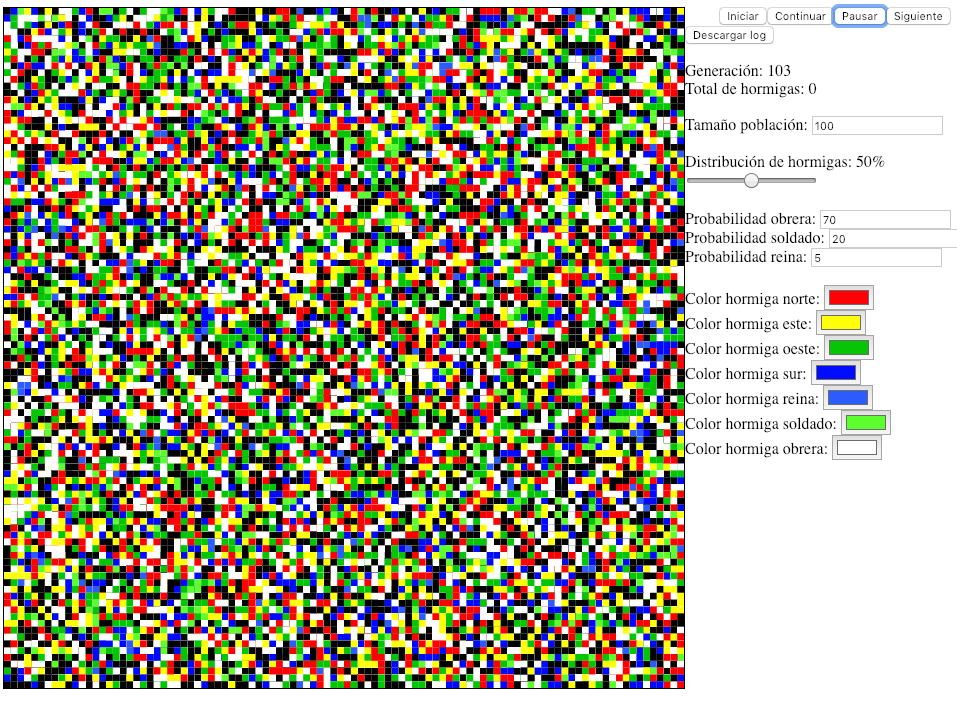
\includegraphics[scale=.3]{HL/img/mod3-1.png}
				\caption{Probabilidades de 75, 20 y 5}
				\label{fig:hl1}
			\end{center}
		\end{figure}

		\begin{figure}[H]
			\begin{center}
				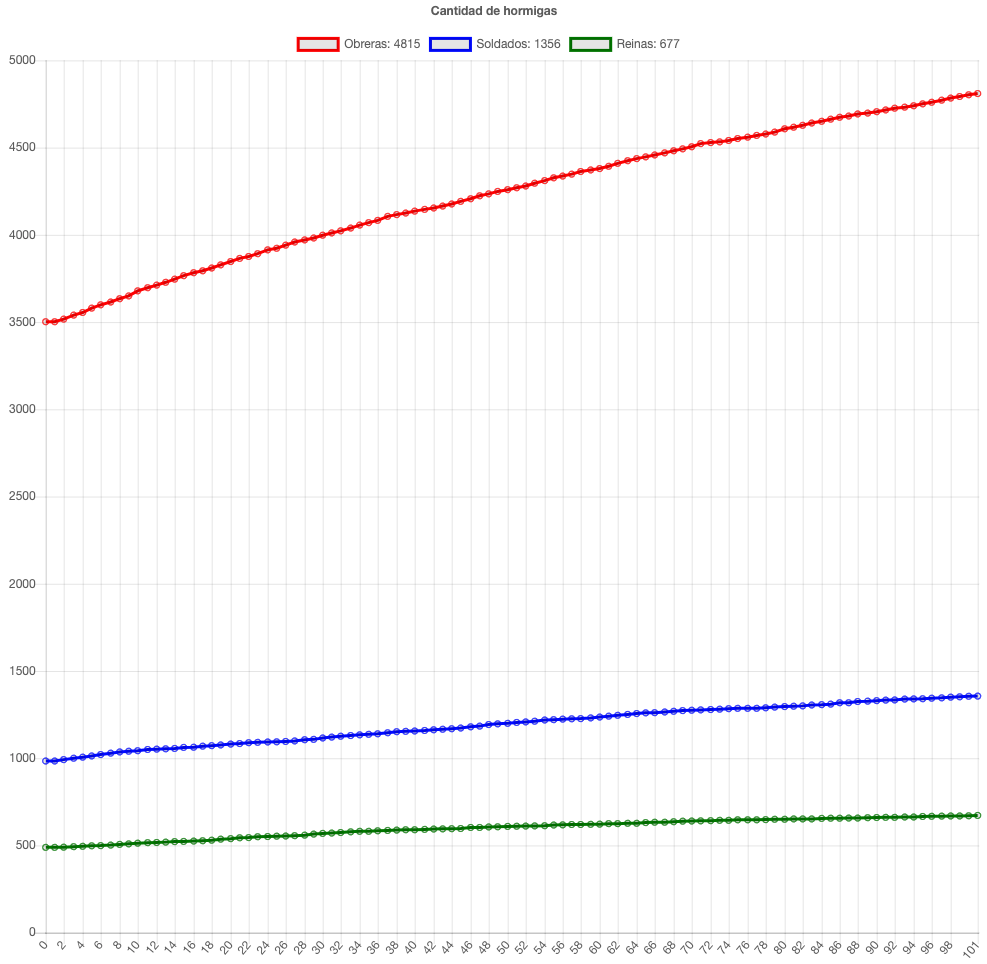
\includegraphics[scale=.24]{HL/img/mod3-2.png}
				\caption{Gráfica de la colonia anterior}
				\label{fig:hl1}
			\end{center}
		\end{figure}

		Como se puede observar, debido a las pocas reinas que existen, es muy complicado que nazcan nuevas hormigas.
